\documentclass[12pt]{article}

\usepackage{sbc-template}
\usepackage{graphicx,url}
\usepackage[utf8]{inputenc}
\usepackage[brazil]{babel}

\usepackage{CJKutf8}
\usepackage{times}            % pacote para usar fonte Adobe Times
% \usepackage[alf,abnt-emphasize=bf]{abntex2cite}	% pacote para usar citações abnt

\usepackage{booktabs}
\usepackage{multirow}
\usepackage{lscape}

\sloppy

\title{Impacto da criptografia da camada de transporte em análises de fluxos com aprendizado de máquina}

\author{
    %Tiago de Carvalho Magnus\inst{1}, Jéferson de Campos Nobre\inst{1} }
}

\address{
%     Instituto de Informática -- Universidade Federal do Rio Grande do Sul
%   (UFRGS)\\
%   Caixa Postal 15.064 -- 91.501-970 -- Porto Alegre -- RS -- Brazil
%   \email{\{tcmagnus,jcnobre\}@inf.ufrgs.br}
}

\begin{document}

\maketitle

\begin{abstract}
    With the increase in the use of cryptography in computer network communications, it is possible that, in the future, encryption of transport layer protocols become commonplace, which may hinder or make automated network flow analysis less efficient. This paper proposes and implements an analysis on the impact of this possible encryption on flow analysis with machine learning. The results showed that the encryption of this network layer could affect, albeit on a small scale, the analysis of network flows. The concepts of explainability and interpretability were used to evaluate the quality of the results.
\end{abstract}

\begin{resumo}
    Com o aumento no uso da criptografia nas comunicações de redes de computadores, é possível que, no futuro, a criptografia dos protocolos da camada de transporte se torne algo comum, o que pode dificultar ou tornar menos eficiente a análise automatizada de fluxos de rede. Este artigo propõe e implementa uma análise sobre o impacto dessa possível criptografia em análises de fluxos com aprendizado de máquina. Os resultados mostraram que a criptografia dessa camada da rede poderia afetar, ainda que em pequena escala, a análise de fluxos de rede. Os conceitos de explicabilidade e interpretabilidade foram utilizados para avaliar a qualidade dos resultados.
\end{resumo}


\section{Introdução}
\label{cap:introducao}

% contexto 1
Existem diversas formas de análise de tráfego de rede, como a inspeção profunda de pacotes (\emph{Deep Packet Inspection}), que analisa o conteúdo detalhado dos pacotes capturados, e a análise de tráfego de rede baseada em fluxos, que analisa o tráfego de rede a partir de fluxos de tráfego extraídos da captura de pacotes. A DPI é mais eficiente que a análise baseada em fluxos, porém, pode ser computacionalmente mais custosa. A análise baseada em fluxos, por sua vez, tende a ser mais eficiente em termos de custo computacional, porém, pode ser menos eficiente em termos de detecção de anomalias e ataques cibernéticos \cite{boukhtouta2016network}.
A análise de tráfego de rede é uma das principais técnicas utilizadas para detectar atividades maliciosas, como malware, ataques de negação de serviço (DDoS), \emph{phishing} e roubo de dados \cite{joshi2015review}.

% contexto 2
A captura de pacotes (pcap), tradicionalmente utilizada no contexto da biblioteca \emph{libpcap}, é uma das principais formas de análise passiva de redes, sendo extensivamente utilizada por administradores de rede e por sistemas de detecção de intrusão (\emph{Intrusion Detection System}) \cite{alias2013study}. A partir da captura de pacotes, é possível extrair informações sobre o tráfego analisado, como o número de \emph{bytes} transferidos, o número de pacotes enviados, o tempo de resposta, entre outros. Essa extração de informações é feita através dos cabeçalhos dos pacotes e do agrupamento dos mesmos em fluxos de tráfego, que são agrupados de acordo com alguma característica, como o endereço IP de origem e destino.

% contexto 3
A detecção de anomalias é uma técnica de análise de dados que busca identificar padrões incomuns ou desvios em relação a um comportamento esperado. Em redes de computadores, a detecção de anomalias pode ser utilizada para identificar atividades suspeitas que possam indicar a presença de um ataque cibernético em andamento. Existem diversas técnicas de detecção de anomalias, como \emph{clustering}, redes neurais e árvores de decisão \cite{usama2019unsupervised}. A detecção de anomalias é frequentemente utilizada em conjunto com técnicas de criptografia de dados e aprendizado de máquina para identificar e mitigar ameaças de segurança em tempo real \cite{bhuyan2013network}.

% contexto 4
A criptografia de dados é uma técnica essencial para garantir a privacidade e segurança das informações que trafegam em redes de comunicação. Porém, a implementação desse tipo de técnica pode interferir na análise de tráfego de rede, que é crucial para a detecção de anomalias e ataques cibernéticos. Recentemente, cada vez mais protocolos da camada de aplicação têm sido criptografados, como a migração do protocolo HTTP para HTTPS, ou a implementação de criptografia no protocolo FTP. Porém, a criptografia de dados em protocolos da camada de transporte, como o protocolo TCP, é ainda pouco explorada, apesar de já possuir propostas de extensão, como visto em \cite{bittau2010case}, \cite{rfc8547} e \cite{rfc8548}, que propõem a aplicação de criptografia oportunística.

% trabalho atual
Apesar da criptografia de dados na camada de aplicação, existem diversas metodologias para, mesmo assim, realizar a análise automatizada de fluxos de tráfego e derivar informações relevantes sobre o tráfego analisado, como qual protocolo está sendo utilizado ou qual aplicação é responsável pelo tráfego gerado \cite{karagiannis2005blinc}. Os autores do \emph{framework} BLINC, por exemplo, afirmam que se os cabeçalhos da camada de transporte fossem criptografados, o tráfego de rede não poderia ser analisado \cite{boutaba2018comprehensive}.

%%%Com o avanço nos desenvolvimentos de algoritmos de aprendizado de máquina, a interpretabilidade dos resultados desses algoritmos tem se tornado um problema cada vez mais importante. Isso porque, embora os algoritmos de aprendizado de máquina sejam capazes de produzir resultados precisos, eles podem se tornar difíceis de entender e explicar, dada a complexidade dos dados analisados e da relação interna entre eles. A falta de transparência em modelos de ML é um desafio significativo, pois pode dificultar a identificação de erros e aprimoramento do modelo \cite{linardatos2020explainable}.

Esse artigo associa as perspectivas mencionadas para entender como a criptografia da camada de transporte nas comunicações de rede poderia afetar a análise automatizada de fluxos de tráfego e a detecção de anomalias a partir dos mesmos. Para isso, foram comparados os resultados obtidos de um modelo de aprendizado supervisionado treinado com fluxos de tráfego de rede não criptografados e de outro treinado com os mesmos fluxos de tráfego de rede, porém, sem as estatísticas obtidas a partir dos cabeçalhos da camada de transporte. Foi utilizado o \emph{framework} SHAP \cite{lundberg2017unified} para apresentar os resultados obtidos de forma mais explicativa.

% estrutura
O artigo está estruturado em 5 seções, incluindo essa introdução, descritos a seguir. Na seção \ref{cap:trabalhos} são apresentados alguns trabalhos relacionados, na seção \ref{cap:analise} é proposta uma solução para realizar a investigação, que tem sua implementação e seus resultados apresentados na seção \ref{cap:implementacao}. Como conclusão, a seção \ref{cap:conclusao} expõe as considerações finais do estudo desenvolvido, além de proposições para possíveis melhorias para essa pesquisa e trabalhos futuros.

% \section{Explicabilidade}
% \label{sec:explicabilidade}

% Com o avanço nos desenvolvimentos de algoritmos de aprendizado de máquina, a interpretabilidade dos resultados desses algoritmos tem se tornado um problema cada vez mais importante. Isso porque, embora os algoritmos de aprendizado de máquina sejam capazes de produzir resultados precisos, eles podem se tornar difíceis de entender e explicar, dada a complexidade dos dados analisados e da relação interna entre eles. A falta de transparência em modelos de ML é um desafio significativo, pois pode dificultar a identificação de erros e aprimoramento do modelo. Diversas técnicas têm sido desenvolvidas para explicar os resultados de modelos de aprendizado de máquina, como o \textit{Local Interpretable Model-agnostic Explanations} (LIME) \cite{ribeiro2016should} ou o \textit{SHapley Additive exPlanations} (SHAP) \cite{linardatos2020explainable}.

% \cite{lundberg2017unified} apresentam uma revisão sobre a interpretabilidade de modelos de aprendizado de máquina a partir do SHAP. De acordo com os autores, a interpretabilidade de modelos de aprendizado de máquina é uma área de pesquisa em desenvolvimento, que tem como objetivo explicar os resultados de modelos de aprendizado de máquina.

% A metodologia presente no SHAP é baseada na teoria dos jogos, e tenta aumentar a interpretabilidade do modelo de máquina ao calcular os valores de importância de cada \textit{feature} para previsões individuais. Os autores propõem os valores SHAP como uma medida unificada da importância das \textit{features}.

% SEÇÃO 2

\section{Trabalhos relacionados}
\label{cap:trabalhos}

Utilizando diversos \textit{datasets}, incluindo o CIC-IDS2017 \cite{sharafaldin2018toward}, \cite{gupta2022cse} apresentam algoritmos de \textit{deep learning} \textit{ensemble} que lidam com o desbalanceamento de classes para o uso em NIDS. Os autores utilizam um sistema multicamadas, com \textit{deep neural networks} (DNN) na primeira, XGBoost na segunda e \textit{random forest} na terceira camada. No CIC-IDS2017, o CSE-IDS proposto pelos autores apresenta acurácia de 92\% e taxa de detecção de ataques (\textit{Attack Detection Rate}) de 98\%.

\cite{al2022dealing} utilizam o XGBoost com os \textit{datasets} NSL-KDD \cite{tavallaee2009detailed} e CIC-IDS2017 para avaliar quais \emph{features} dos conjuntos de dados são mais relevantes para a classificação de tráfego, através das metodologias de \emph{feature selection} e \emph{oversampling}. Os autores relatam que o uso de estratégias de \emph{OneVsRest (OVR)} com o XGBoost apresenta melhores resultados, com acurácia acima de 99\% e \emph{f1 score} de 87\% no CIC-IDS2017.

Em \cite{le2022classification}, é feita uma análise sobre como as \emph{features} dos fluxos de rede afetam o desempenho de algoritmos de aprendizado de máquina para detecção de anomalias, através da explicabilidade. Os autores utilizam os \emph{datasets} IotIDS20 \cite{ullah2020scheme} e NetFlow IoT V2 \cite{sarhan2022towards}, que contém fluxos de rede de dispositivos IoT. Os autores utilizam a técnica de \emph{ensemble} com algoritmos de DT e RF e, em seguida, utilizam explicações locais e explicações globais do SHAP para analisar a importância das \emph{features} para a classificação.
%%%Analisando os diagramas SHAP gerados pelos autores, é possível notar que o algoritmo de DT considera que a porta de destino, o \emph{timestamp} e o identificador do fluxo (\emph{Flow\_ID}) impactam positivamente para classificar um tráfego como anomalia, com até cerca de 60 instâncias. Após isso, essas mesmas \emph{features} passam a impactar negativamente. O inverso acontece na classificação de tráfego como benigno. Além disso, na classificação de tráfego de ataque DoS, os autores observam que, com muitas instâncias, o algoritmo de RF depende do protocolo de aplicação (\emph{L7\_PROTO}) para classificar o tráfego como ataque.

% SEÇÃO 3

\section{Análise proposta}
\label{cap:analise}

A eficiência de sistemas de detecção de intrusão e da segurança de redes dependem da velocidade em que ataques e ameaças são detectados. Por isso, conjuntos de tráfego de rede são extremamente necessários para o melhor desempenho das ferramentas utilizadas \cite{dijkhuizen2018survey}. Dentre os conjuntos de dados publicamente disponíveis, foi selecionado o CIC-IDS2017 \cite{sharafaldin2018toward} pois, além da captura de pacotes, o \emph{dataset} também possui o fluxo de tráfego da rede, que é o que será utilizado nessa análise. Os fluxos de rede anômalos foram gerados a partir de um conjunto de ataques de intrusão, como \emph{Brute Force}, \emph{Heartbleed}, \emph{Botnet}, \emph{Denial of Service (DoS)}, \emph{Distributed Denial of Service (DDoS)}, \emph{PortScan} e um conjunto de ataques \emph{web}, como \emph{SQL Injection} e \emph{Cross-site scripting (XSS)}. \cite{rosay2022multi} discutem em mais detalhes as \textit{features} e os ataques disponibilizados no \emph{dataset} CIC-IDS2017.

Os fluxos de rede do CIC-IDS2017 possuem informações detalhadas sobre a direção dos pacotes enviados. Portanto, algumas \textit{features} do \emph{dataset} possuem os prefixos \textit{bwd} e \textit{fwd}, que indicam, respectivamente, pacotes que foram enviados de um cliente para um servidor (uma requisição) ou do servidor para o cliente, a resposta para uma requisição. Por exemplo, a \textit{feature} \textit{fwd\_pkt\_len\_max} indica o tamanho máximo dos pacotes enviados do cliente para o servidor, enquanto a \textit{feature} \textit{bwd\_pkt\_len\_max} indica o tamanho máximo dos pacotes enviados do servidor para o cliente.

\subsection{Tratamento dos dados}
\label{sec:tratamento}

Apesar de ser um conjunto de dados bastante completo, o CIC-IDS2017 possui alguns problemas, como dados inválidos ou duplicados e incoerência nos rótulos (\emph{labelling}) de alguns fluxos. Para corrigir esses problemas, \cite{rosay2021cic} criaram o \emph{dataset} LYCOS2017, que é uma versão corrigida do CIC-IDS2017. Dentre as correções feitas, estão a remoção de \emph{features} duplicadas, a correção nos cálculos de algumas \emph{features}, a contagem dos tamanhos dos pacotes e o uso das \textit{flags} TCP.

Após a correção dos dados, o \emph{dataset} LYCOS2017 possui quatorze classificações possíveis para os fluxos, que são: \emph{benign}, \emph{bot}, \emph{ddos}, \emph{dos\_goldeneye}, \emph{dos\_hulk}, \emph{dos\_slowhttptest}, \emph{dos\_slowloris}, \emph{ftp\_patator}, \emph{heartbleed}, \emph{portscan}, \emph{ssh\_patator}, \emph{webattack\_bruteforce}, \emph{webattack\_sql\_injection} e \emph{webattack\_xss}. Cada fluxo de rede possui 84 atributos, sendo que 83 deles são numéricos. O atributo restante é a classificação do fluxo, que foi utilizado para treinar o modelo de aprendizado de máquina de forma supervisionada nessa análise.

\subsection{Criptografia da camada de transporte}
\label{sec:criptografia}

Os dados da camada de transporte são encontrados nos campos \emph{source port}, \emph{destination port}, \emph{sequence number}, \emph{acknowledgement number}, \emph{flags}, \emph{window size}, \emph{urgent pointer} e \emph{options}. Os dados relativos a esses campos serão ofuscados através da remoção das estatísticas de fluxo geradas a partir deles.

Para simular a criptografia dos dados relativos à camada de transporte, foi feita uma análise das \textit{features} estatísticas que foram obtidas através desses dados. Os dados e estatísticas removidas do \textit{dataset} original são:

\begin{itemize}
    \item \emph{src\_port} e \emph{dst\_port}: os números de portas de origem e destino dos fluxos de rede. Esses números são utilizados para identificar os processos que estão enviando e recebendo os dados;
    \item \emph{fwd\_tcp\_init\_win\_bytes} e \emph{bwd\_tcp\_init\_win\_bytes}: o tamanho da janela TCP inicial do fluxo de rede.
    \item \emph{flag\_rst}, \emph{flag\_urg}, \emph{flag\_ack}, \emph{flag\_psh}, \emph{flag\_syn}, \emph{flag\_fin}, \emph{flag\_cwr} e \emph{flag\_ece}: a quantidade de pacotes que possuem cada uma das \emph{flags} de controle de fluxo do TCP, independente da direção do fluxo de comunicação.
    \item \emph{fwd\_flag\_urg} e \emph{bwd\_flag\_urg}: a quantidade de pacotes que possuem a \emph{flag} de urgência do TCP, na direção do fluxo de comunicação.
    \item \emph{fwd\_flag\_psh} e \emph{bwd\_flag\_psh}: a quantidade de pacotes que possuem a \emph{flag} de \emph{push} do TCP, na direção do fluxo de comunicação.
\end{itemize}

Dessa forma, os conjuntos de dados gerados a partir da remoção das estatísticas de fluxo possuem 76 atributos, incluindo o rótulo de classificação.

Embora os dados relativos à camada de transporte sejam criptografados, camadas inferiores do modelo OSI também possuem informações sobre o tamanho do pacote, portanto, não é possível remover estatísticas como a quantidade de \emph{bytes} e de pacotes em um fluxo de rede. Vale ressaltar que, até a versão responsável por gerar o CIC-IDS2017, o CICFlowMeter não gerava estatísticas com os dados de camadas superiores à de transporte, como a camada de aplicação, por exemplo.

\subsection{Definição do modelo}
\label{sec:modelo}

Para definir qual o melhor algoritmo e quais os melhores parâmetros para ele, foi utilizado o \emph{framework} H2O \cite{h2oai}. Executando a ferramenta \emph{AutoML} do H2O, foi obtida uma tabela com os \emph{scores} de cada algoritmo testado. O modelo a utilizado foi o que obteve o melhor \emph{score} na métrica \emph{mean\_per\_class\_error} (erro médio por classe), que é a métrica utilizada para comparar o desempenho de modelos de classificação multinomial \cite{h2oai}.

Após obter o melhor algoritmo e parâmetros para os conjuntos de dados de treinamento e validação, foi possível obter os \emph{scores} de cada modelo a partir dos dados de teste, que foram utilizados para comparação com os resultados obtidos pelos autores do \emph{dataset} LYCOS2017.

\subsection{Comparação de resultados}
\label{sec:comparacao}

Para fins de comparação, tanto os autores do \emph{dataset} LYCOS2017 quanto este trabalho usam as matrizes de confusão global dos modelos gerados. A partir dessas matrizes, diversas métricas estatísticas podem ser obtidas. Dentre elas, estão a taxa de verdadeiros positivos (TPR), a taxa de falsos positivos (FPR), a taxa de verdadeiros negativos (TNR), a taxa de falsos negativos (FNR), a acurácia  (\emph{accuracy}), a precisão (\emph{precision}), a revocação (\emph{recall}), a medida F1 (\emph{f1 score}) e o coeficiente de correlação de Matthews (MCC) \cite{h2oai}.

Através da comparação dos \emph{scores} dos modelos criados nesse trabalho, é possível verificar se a criptografia dos dados da camada de transporte afeta, de forma significativa, o desempenho do modelo na detecção de atividades anômalas de rede.

\section{Implementação e avaliação}
\label{cap:implementacao}

Os conjuntos de dados do LYCOS2017 já haviam sido separados previamente em conjuntos de treinamento, validação e teste por \cite{rosay2021cic}, que os separou em porções de 50\%, 25\% e 25\%, respectivamente. Após o tratamento e criação dos dados criptografados, conforme descrito nas seções \ref{sec:tratamento} e \ref{sec:criptografia}, foi utilizado o \emph{framework} H2O para identificar os melhores modelos de aprendizado de máquina para o \emph{dataset} analisado, assim como seus respectivos \emph{scores}. Ordenando o desempenho pela métrica \emph{mean\_per\_class\_error}, o modelo de XGBoost obteve o melhor desempenho, seguido do modelo de GBM, ambos são modelos de \emph{ensemble} de árvores de decisão. Nessa análise, o modelo de XGBoost será considerado o principal modelo a ser utilizado, enquanto que o modelo de GBM será utilizado apenas para efeitos de comparação.

Os parâmetros usados com o \emph{AutoML} do H2O são apresentados abaixo:

\begin{itemize}
    \item \emph{max\_runtime\_secs=600}: limita a execução do \emph{AutoML} a 10 minutos.
    \item \emph{max\_models=3}: limita o número de modelos a serem treinados para focar em desenvolver modelos melhores.
    \item \emph{sort\_metric=mean\_per\_class\_error}: ordena os modelos de acordo com a métrica de avaliação.
    \item \emph{seed=6898}: define uma semente para a geração de números aleatórios para garantir a reprodutibilidade.
\end{itemize}

Os demais parâmetros foram definidos com os valores padrão do \emph{AutoML}. Maiores detalhes sobre os parâmetros do \emph{AutoML} podem ser encontrados na documentação oficial do H2O \cite{h2oai}.

Apesar de obter resultados satisfatórios com o H2O, foi identificado posteriormente que o \emph{framework} não possui a ferramenta de explicabilidade SHAP para classificação multinomial. Por esse motivo, os modelos de XGBoost foram traduzidos para o \emph{framework} scikit-learn, que possui maior suporte para a ferramenta SHAP. Após a conversão, o desempenho dos modelos foi comparado e os resultados obtidos foram equivalentes.

\subsection{Resultados obtidos}
\label{sec:resultados}

Ao aplicar os modelos de aprendizado de máquina nos seus respectivos \emph{datasets} de teste, foi possível obter as matrizes de confusão resumidas, que são apresentadas na tabela \ref{tab:cm_completo} e na tabela \ref{tab:cm_criptografado}.

É importante ressaltar que, em \cite{rosay2021cic}, uma classe considerada positiva foi definida como uma classe que corresponde a um ataque ou tráfego anômalo na rede, enquanto que uma classe considerada negativa foi definida como uma classe que corresponde ao tráfego benigno na rede. Os mesmos critérios foram utilizados para definir as classes positivas e negativas para os modelos apresentados neste trabalho.

\begin{table}[h]
    \centering
    \begin{tabular}{l|l|c|c|c}
        \multicolumn{2}{c}{}&\multicolumn{2}{c}{Classe predita}&\\
        \cline{3-4}
        \multicolumn{2}{c|}{}&Positivo&Negativo&\multicolumn{1}{c}{Total}\\
        \cline{2-4}
        \multirow{2}{*}{Classe real}& Positivo & $110034$ & $13$ & $110047$\\
        \cline{2-4}
        & Negativo & $16$ & $110142$ & $110158$\\
        \cline{2-4}
        \multicolumn{1}{c}{} & \multicolumn{1}{c}{Total} & \multicolumn{1}{c}{$110050$}
        & \multicolumn{1}{c}{$110155$}\\
    \end{tabular}
    \caption{Matriz de confusão do modelo de XGBoost com os dados completos}
    \label{tab:cm_completo}
\end{table}

\begin{table}[h]
    \centering
    \begin{tabular}{l|l|c|c|c}
        \multicolumn{2}{c}{}&\multicolumn{2}{c}{Classe predita}&\\
        \cline{3-4}
        \multicolumn{2}{c|}{}&Positivo&Negativo&\multicolumn{1}{c}{Total}\\
        \cline{2-4}
        \multirow{2}{*}{Classe real}& Positivo & $109896$ & $30$ & $109926$\\
        \cline{2-4}
        & Negativo & $80$ & $110078$ & $110158$\\
        \cline{2-4}
        \multicolumn{1}{c}{} & \multicolumn{1}{c}{Total} & \multicolumn{1}{c}{$109976$}
        & \multicolumn{1}{c}{$110108$}\\
    \end{tabular}
    \caption{Matriz de confusão do modelo de XGBoost com os dados criptografados}
    \label{tab:cm_criptografado}
\end{table}


Com base nas matrizes de confusão, foi possível obter os resultados estatísticos apresentados na tabela \ref{tab:resultados}.

\begin{table}[h!]
    \resizebox{\textwidth}{!}{%
    \begin{tabular}{@{}llrrrrrr@{}}
        \toprule
        \textbf{Algoritmo} &
        \textit{\textbf{Dataset}} &
        \multicolumn{1}{l}{\textit{\textbf{Accuracy (\%)}}} &
        \multicolumn{1}{l}{\textit{\textbf{Precision (\%)}}} &
        \multicolumn{1}{l}{\textit{\textbf{Recall (\%)}}} &
        \multicolumn{1}{l}{\textit{\textbf{f1 score (\%)}}} &
        \multicolumn{1}{l}{\textit{\textbf{False Positive Rate (\%)}}} &
        \multicolumn{1}{l}{\textit{\textbf{MCC}}} \\ \midrule
        XGBoost & Completo      & 99,9868 & 99,9855 & 99,9882 & 99,9861 & 0,00145 & 0.999737 \\
        XGBoost & Criptografado & 99,9500 & 99,9273 & 99,9727 & 99,9500 & 0,00726 & 0.999000 \\
        GBM     & Completo      & 99,9764 & 99,9764 & 99,9764 & 99,9764 & 0,00236 & 0.999528 \\
        GBM     & Criptografado & 99,9382 & 99,9127 & 99,9636 & 99,9382 & 0,00871 & 0.998764 \\ \bottomrule
    \end{tabular}%
    }
    \caption{Resultados obtidos pelo autor}
    \label{tab:resultados}
\end{table}

Com esses resultados, é possível observar que, em ambos os algoritmos, os modelos de GBM e XGBoost obtiveram resultados ligeiramente divergentes entre os \emph{datasets} completos e criptografados. No entanto, os resultados obtidos de todos os modelos foram satisfatórios, com acurácia, precisão, \emph{recall} e \emph{f1 score} superiores a 99,9\%, e MCC superior a 99,8\%.

Utilizando esses dados e os resultados obtidos pelos autores do LYCOS2017, foi possível obter uma comparação entre os resultados obtidos pelos dois \emph{datasets}, conforme apresentado na figura \ref{fig:model_comparison}.

\begin{figure}[h!]
    \centering
    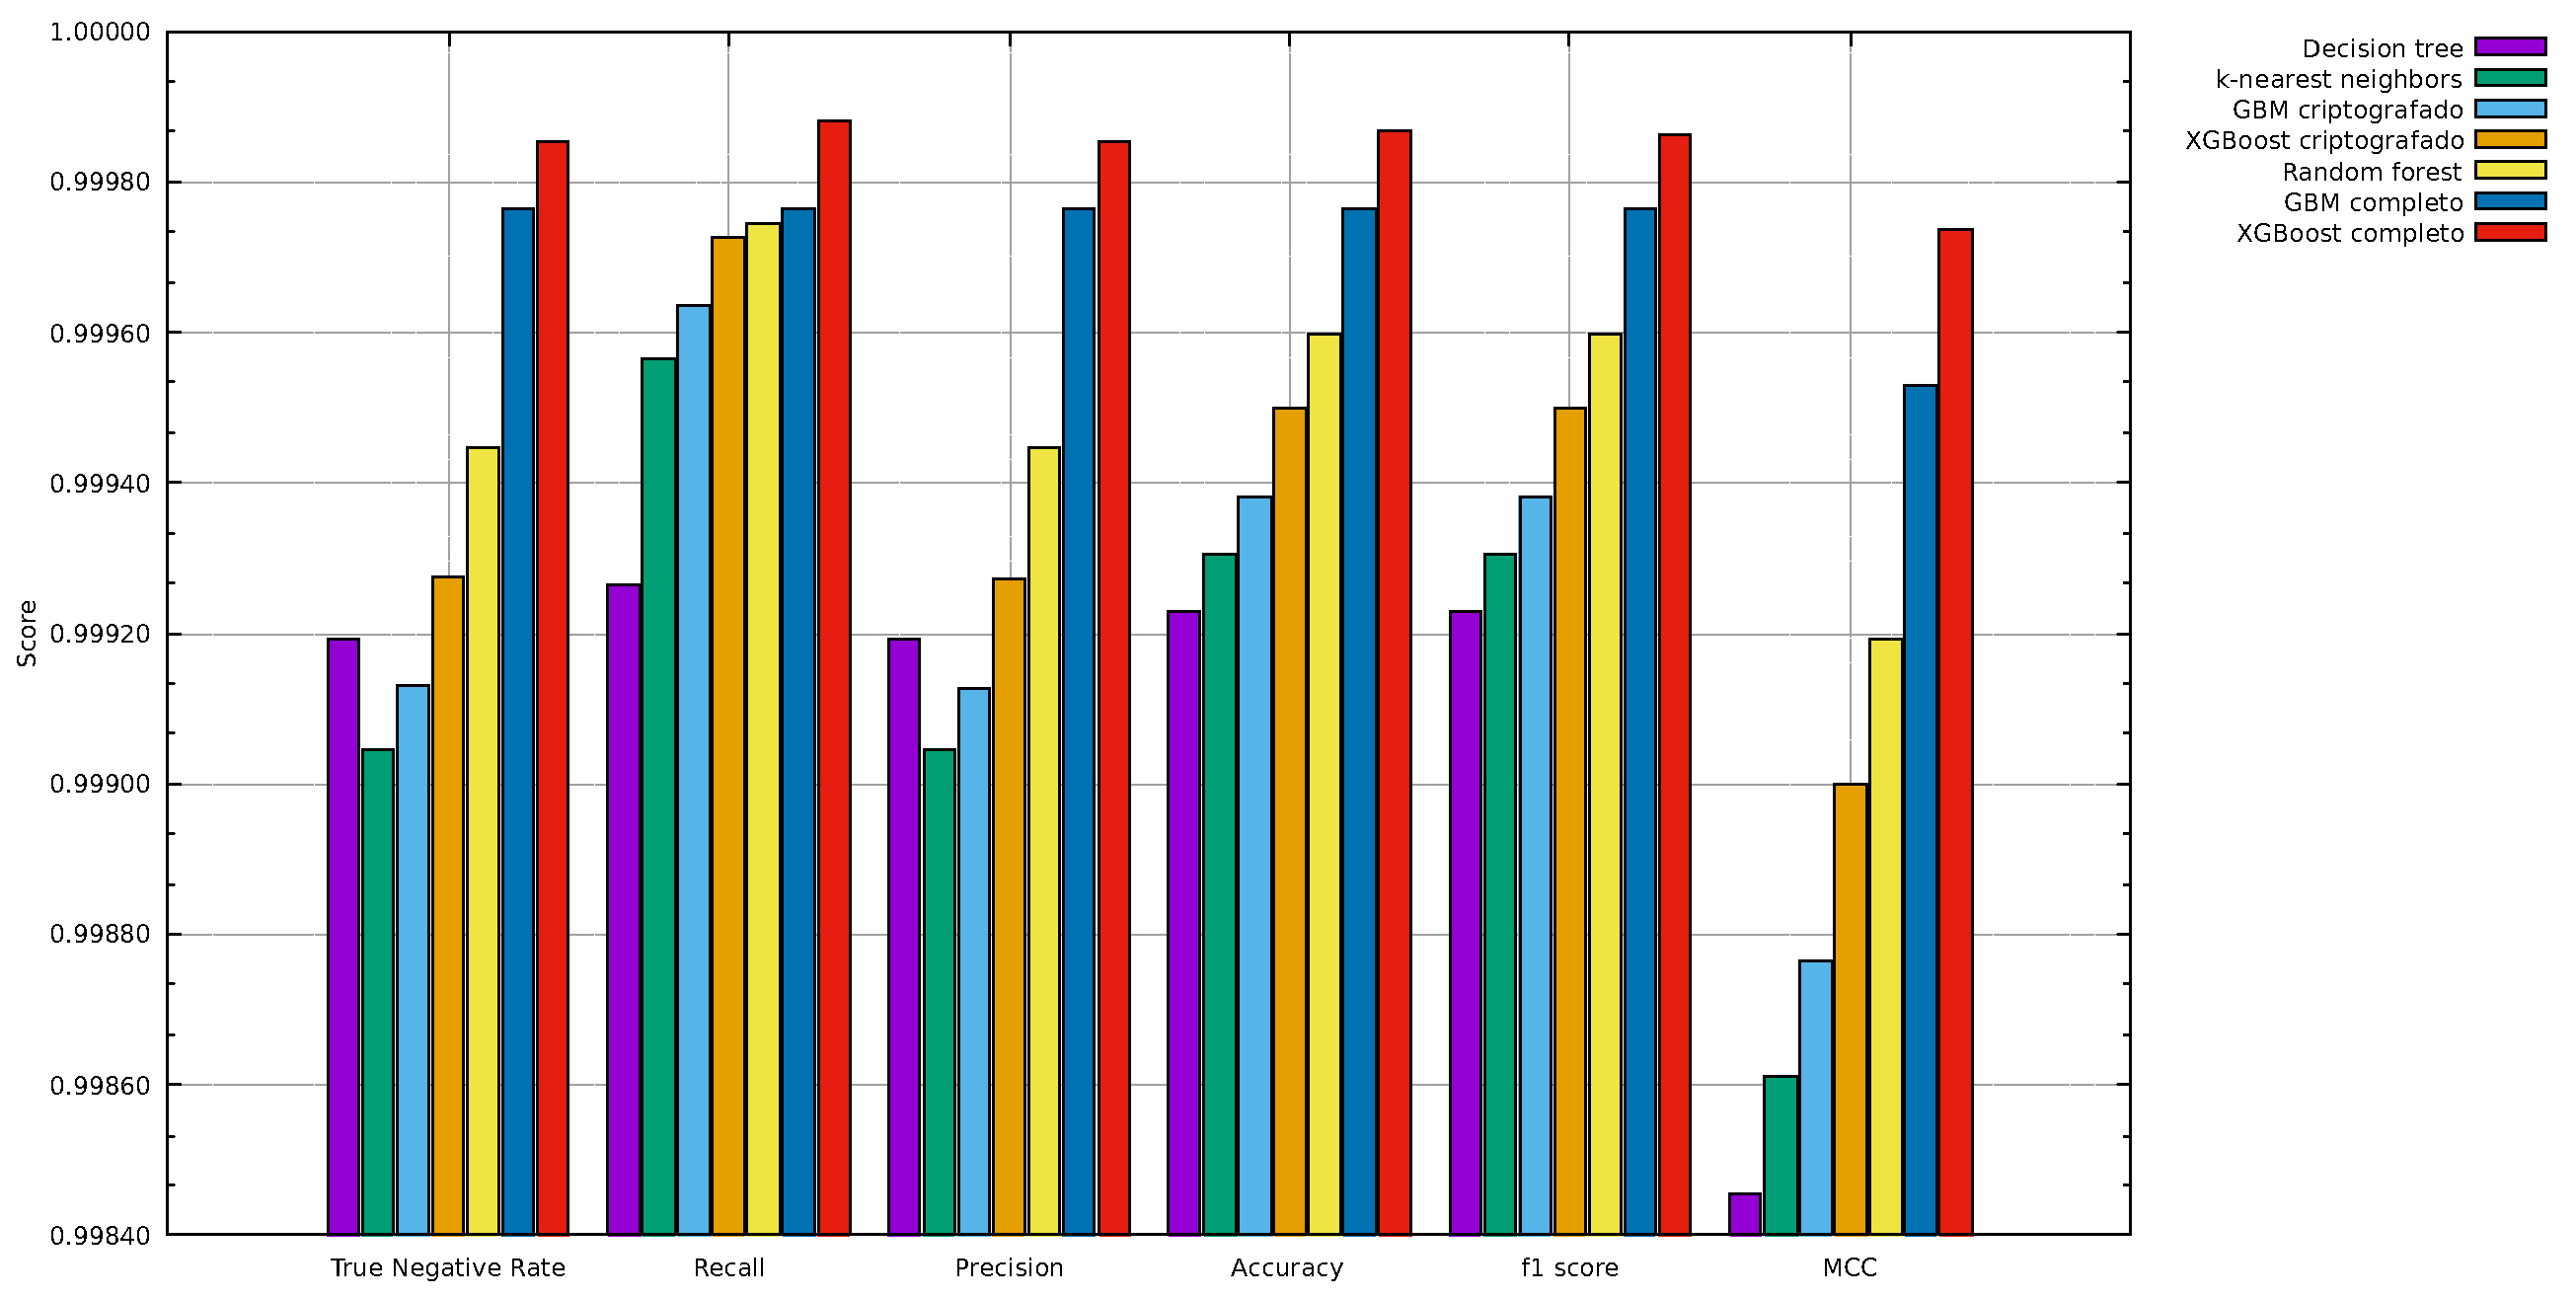
\includegraphics[width=0.8\textwidth]{figures/model_comparison.pdf}
    \caption{Comparação entre os resultados obtidos pelos autores do LYCOS2017 e o autor}
    \label{fig:model_comparison}
\end{figure}

Apesar da alta performance dos modelos de GBM e XGBoost, é importante observar que o \emph{dataset} de base utilizado por \cite{rosay2021cic} é, propositalmente, um \emph{dataset} com um enorme desbalanceamento entre as classes, principalmente entre o tráfego benigno e o tráfego anômalo, como forma de simular uma rede de computadores real \cite{ring2019survey}. Por esse motivo, pequenas variações nas taxas de detecção de tráfego anômalo podem representar um impacto significativo no desempenho real do modelo.

\subsection{Análise e explicação dos resultados}
\label{sec:resultados_explicabilidade}
% Descrever a análise dos resultados obtidos com o SHAP.

Através do SHAP, foi possível obter uma análise mais detalhada dos resultados dos modelos de XGBoost. As figuras \ref{fig:features_completo} e \ref{fig:features_criptografado} apresentam os gráficos de sumário SHAP, que distribuem a importância de cada \emph{feature}, por classe, na predição do modelo.

\begin{figure}[h!]
    \centering
    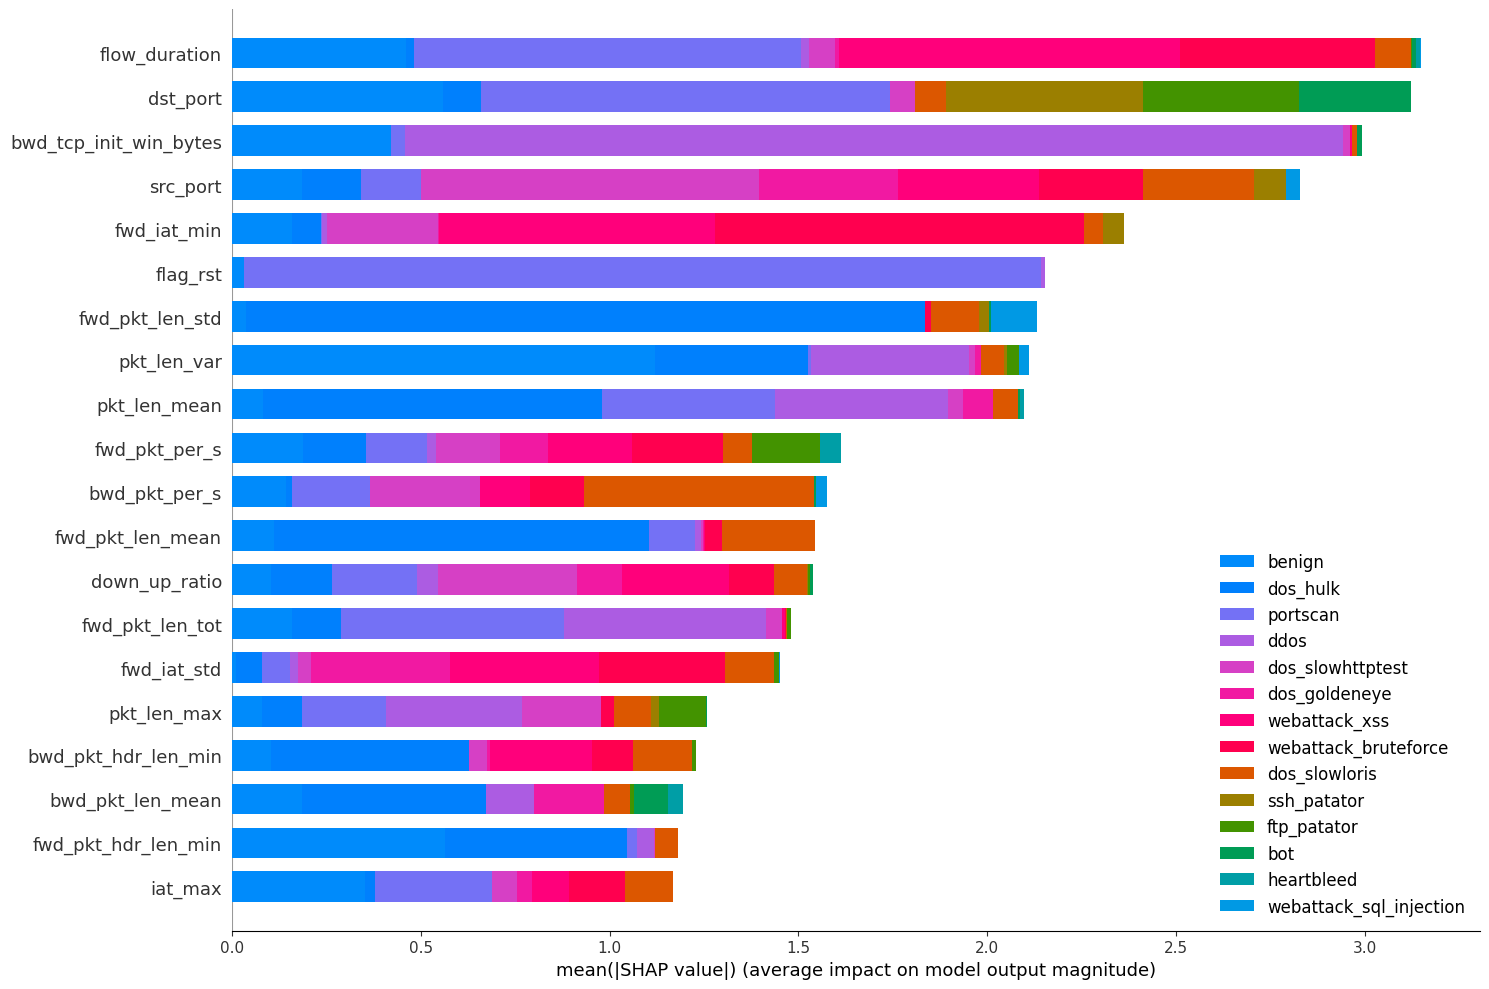
\includegraphics[width=0.8\textwidth]{figures/feature_importance_completo.png}
    \caption{Importância das features por classe - dataset completo}
    \label{fig:features_completo}
\end{figure}

No gráfico de sumário SHAP do modelo treinado com o \emph{dataset} completo, é possível observar que as \emph{features} relacionadas aos dados da camada de transporte, como porta de destino (\textit{dst\_port}) e a porta de origem (\textit{src\_port}), são bastante presentes entre as \emph{features} mais importantes. Porém, \emph{features} de metadados dos fluxos, como duração do fluxo e o intervalo entre pacotes são importantes para a detecção de alguns ataques, como DDoS e de ataques web.

\begin{figure}[h!]
    \centering
    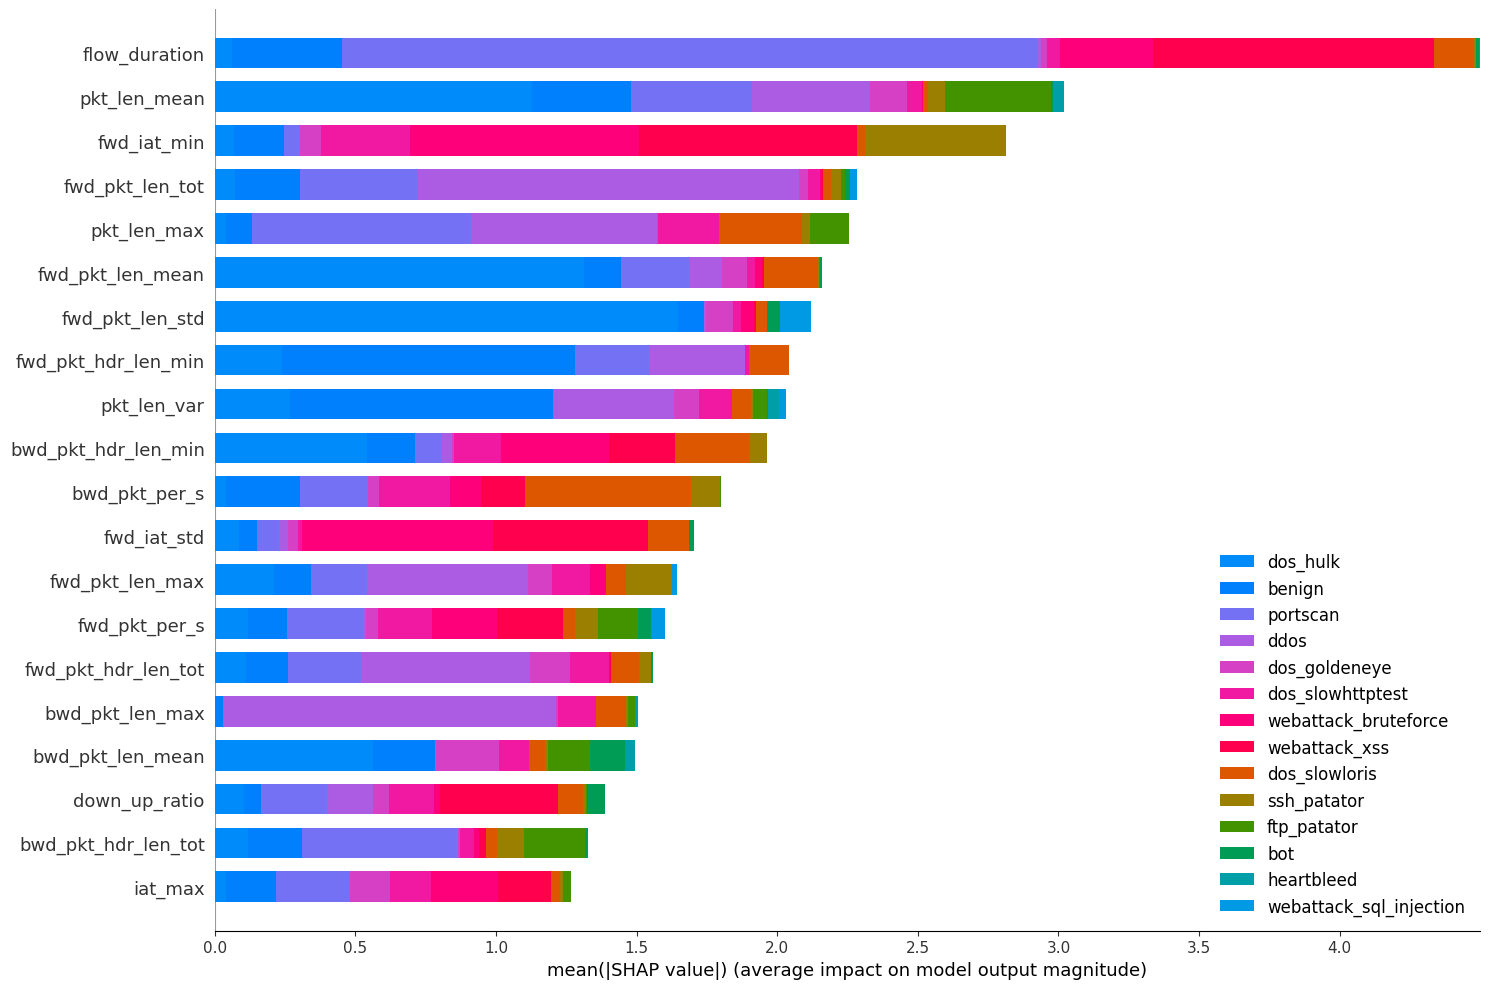
\includegraphics[width=0.8\textwidth]{figures/feature_importance_criptografado.png}
    \caption{Importância das features por classe - dataset criptografado}
    \label{fig:features_criptografado}
\end{figure}

Já no gráfico de sumário SHAP do modelo treinado com o \emph{dataset} criptografado, podemos notar que a \emph{feature} de duração do fluxo se mantém como a mais importante, enquanto que as \emph{features} relacionadas à variação de tamanho de pacotes e cabeçalhos dos pacotes dominam na detecção de todos os tipos de tráfego. Um detalhe importante é que \emph{features} que tinham pouca importância para o modelo com dados completos, como o tamanho mínimo dos headers dos pacotes da origem do fluxo (\textit{fwd\_pkt\_hdr\_len\_min}) e o tamanho máximo dos pacotes no fluxo (\textit{pkt\_len\_max}), passam a ser importantes para o modelo com dados criptografados. Essa mudança pode indicar uma dependência entre as \emph{features}, que pode ser explorada para melhorar a performance dos modelos.

Nas subseções a seguir, serão apresentados os gráficos de sumário SHAP para cada classe, com as \emph{features} mais importantes para a classificação de cada fluxo como tráfego de determinado ataque ou tráfego benigno. Nesses gráficos, as \emph{features} são ordenadas de acordo com a importância para a classificação de cada fluxo, e as cores indicam o valor de cada \emph{feature} para o fluxo em questão. As cores mais azuis indicam valores mais baixos, enquanto as cores mais avermelhadas indicam valores mais altos. Além disso, a posição de cada ponto no gráfico indica o valor SHAP da \emph{feature} para aquele fluxo, sendo que valores mais altos indicam que a \emph{feature} teve um impacto positivo na sua classificação, enquanto valores mais baixos indicam que a \emph{feature} teve um impacto negativo na mesma classificação.

\subsubsection{Detecção de tráfego benigno}
\label{subsec:benigno}

Na detecção de tráfego benigno, as figuras \ref{fig:summary_benigno_completo} e \ref{fig:summary_benigno_criptografado} apresentam quais \emph{features} impactam mais na classificação de um fluxo como tráfego benigno.

\begin{figure}[h!]
    \centering
    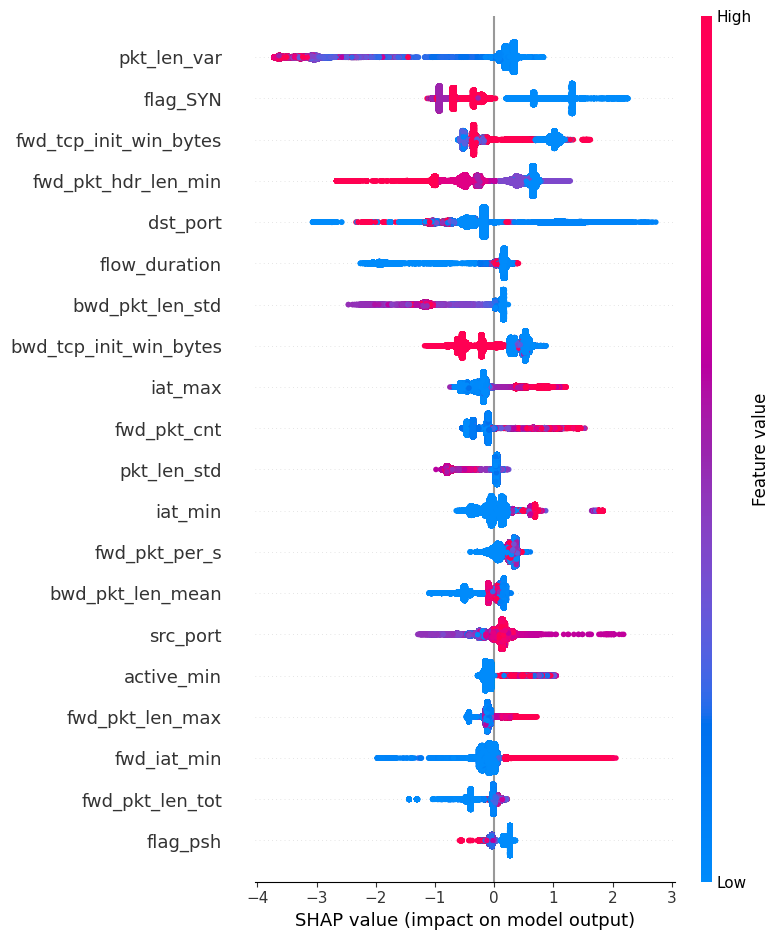
\includegraphics[width=0.8\textwidth]{figures/summary_benigno_completo.png}
    \caption{Impacto das features na detecção de tráfego benigno - dataset completo}
    \label{fig:summary_benigno_completo}
\end{figure}

No \emph{dataset} completo, podemos notar como que algumas \emph{features} da camada de transporte impactam na classificação de um tráfego como benigno. Baixas quantidades da \textit{flag} de sincronização (\textit{flag\_SYN}) na comunicação fornecem um \textit{score} mais alto para a predição de tráfego benigno, assim como a presença de \textit{src\_port} mais altas. É interessante notar que a simples presença de algumas \emph{features}, independente do seu valor, impactam positivamente na classificação de um fluxo como benigno, como a quantidade de \textit{bytes} na janela de iniciação da comunicação TCP da origem do fluxo (\textit{fwd\_tcp\_init\_win\_bytes}).

\begin{figure}[h!]
    \centering
    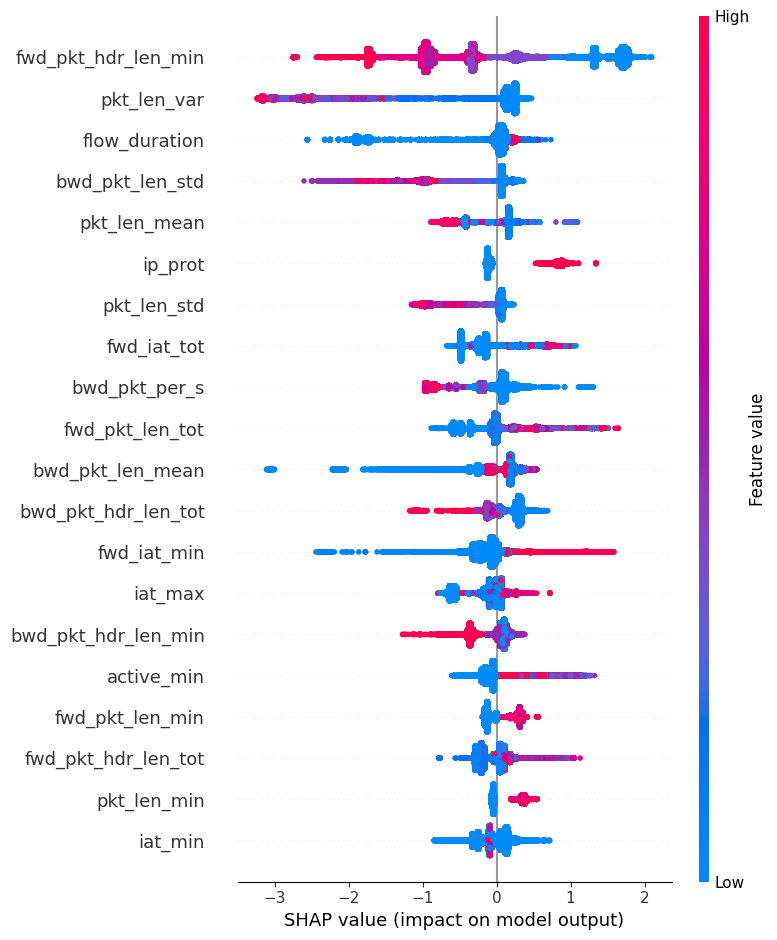
\includegraphics[width=0.8\textwidth]{figures/summary_benigno_criptografado.png}
    \caption{Impacto das features na detecção de tráfego benigno - dataset criptografado}
    \label{fig:summary_benigno_criptografado}
\end{figure}

No \emph{dataset} criptografado, os valores estatísticos das \emph{features} passam a ser mais importantes para a classificação de um fluxo como benigno. Por exemplo, fluxos com \textit{fwd\_pkt\_hdr\_len\_min} mais altas e mais baixas impactam de forma positiva e negativa, respectivamente, na classificação de um fluxo como benigno. Além disso, valores altos das \emph{features} do tipo de protocolo IP (\textit{ip\_prot}), o intervalo mínimo entre a chegada de pacotes no destino (\textit{fwd\_iat\_min}) e o \textit{pkt\_len\_min} impactam positivamente.

\subsubsection{Detecção de ataques DDoS}
\label{subsec:ddos}

Para a detecção de DDoS, as figuras \ref{fig:summary_ddos_completo} e \ref{fig:summary_ddos_criptografado} apresentam quais \emph{features} impactam mais na classificação de um fluxo como DDoS. Nesse tipo de ataque, é possível notar que o tamanho dos pacotes é a \emph{feature} mais importante para a classificação de um fluxo como DDoS, tanto no \emph{dataset} completo quanto no \emph{dataset} criptografado.

\begin{figure}[h!]
    \centering
    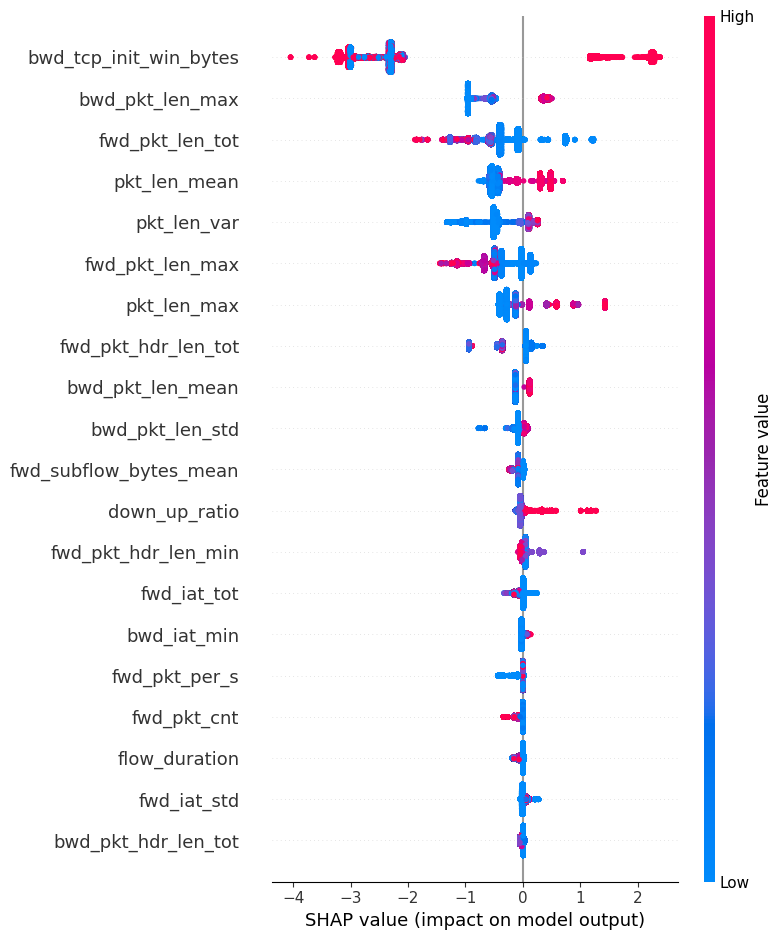
\includegraphics[width=0.8\textwidth]{figures/summary_ddos_completo.png}
    \caption{Impacto das features na detecção de DDoS - dataset completo}
    \label{fig:summary_ddos_completo}
\end{figure}

Com o \emph{dataset} completo, notamos que fluxos com \textit{bwd\_pkt\_len\_max} mais altos impactam positivamente na classificação de um fluxo como DDoS. No entanto, o valores mais altos do tamanho máximo dos pacotes na direção oposta (\textit{fwd\_pkt\_len\_max}) impacta negativamente na classificação de um fluxo como DDoS. Uma \emph{feature} que chama atenção é a \textit{bwd\_tcp\_init\_win\_bytes}, que fica nos extremos dos valores SHAP, indicando que valores altos da \emph{feature} impactam positiva e negativamente, apesar de valores baixos da \emph{feature} impactarem somente de forma negativa. Essa variação de impacto reforça a ideia de que há uma relação de dependência entre as \emph{features}, dependendo dos seus valores.

\begin{figure}[h!]
    \centering
    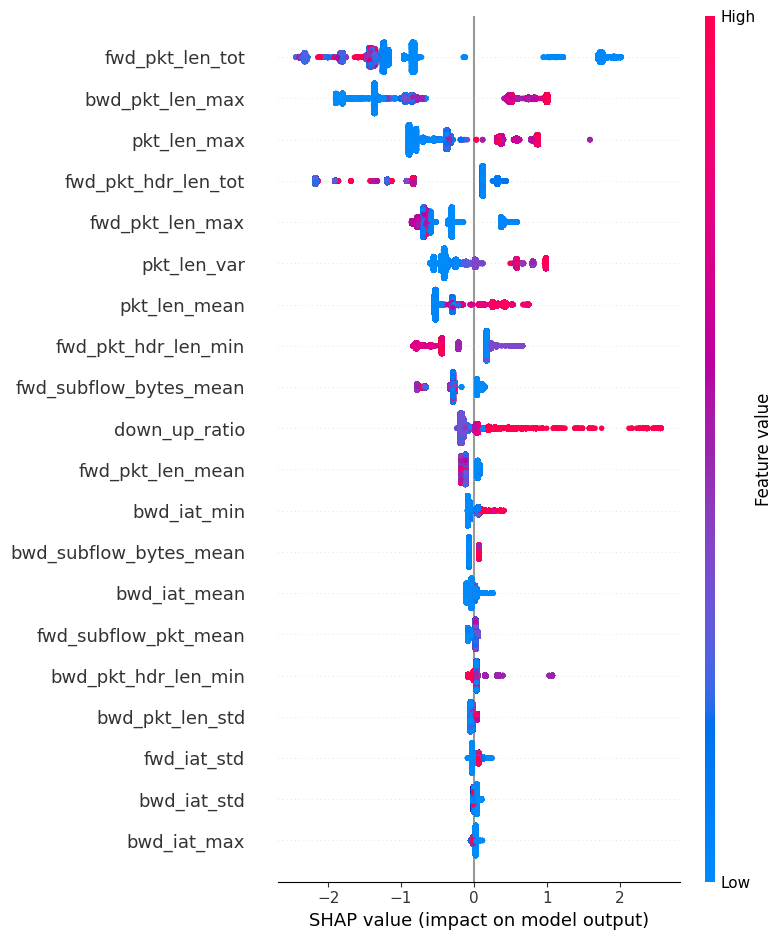
\includegraphics[width=0.8\textwidth]{figures/summary_ddos_criptografado.png}
    \caption{Impacto das features na detecção de DDoS - dataset criptografado}
    \label{fig:summary_ddos_criptografado}
\end{figure}

Sem os dados da camada de transporte, as \emph{features} direcionais dominam na classificação de um fluxo como DDoS. Por exemplo, fluxos com \textit{fwd\_pkt\_len\_max} mais altos impactam negativamente na classificação de um fluxo como DDoS, enquanto que fluxos com \textit{bwd\_pkt\_len\_max} mais altos impactam positivamente.

Em ambos os casos, altos valores da \textit{feature} da razão entre download e upload de pacotes (\textit{down\_up\_ratio}) indicam fortemente que um fluxo é do tipo DDoS.

% \subsubsection{Detecção de ataques portscan}
% \label{subsec:portscan}

% Para a detecção de \emph{portscan}, as figuras \ref{fig:summary_portscan_completo} e \ref{fig:summary_portscan_criptografado} apresentam quais \emph{features} impactam mais na classificação de um fluxo como \emph{portscan}. Nesse tipo de ataque, a porta de destino, o uso da \textit{flag rst} e a duração do fluxo (\textit{flow\_duration}) são as \emph{features} mais importantes para classificar um fluxo como um ataque de \emph{portscan}.

% \begin{figure}[]
%     \centering
%     \caption{Impacto das features na detecção de portscan - dataset completo}
%     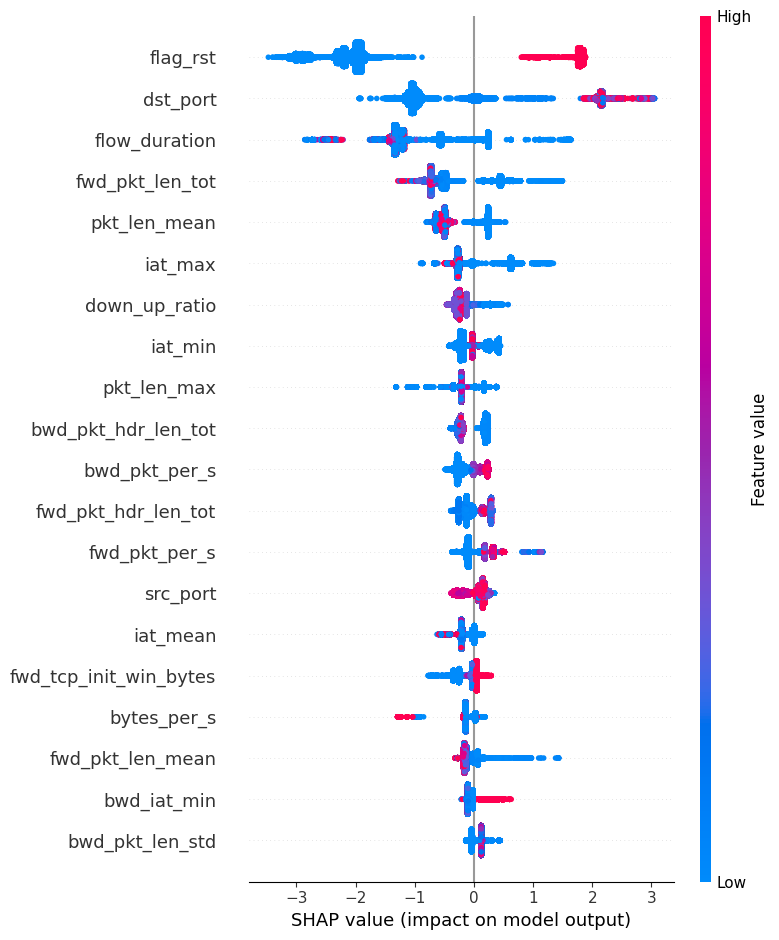
\includegraphics[width=0.8\textwidth]{figures/summary_portscan_completo.png}
%     \caption*{Fonte: O autor}
%     \label{fig:summary_portscan_completo}
% \end{figure}

% \begin{figure}[]
%     \centering
%     \caption{Impacto das features na detecção de portscan - dataset criptografado}
%     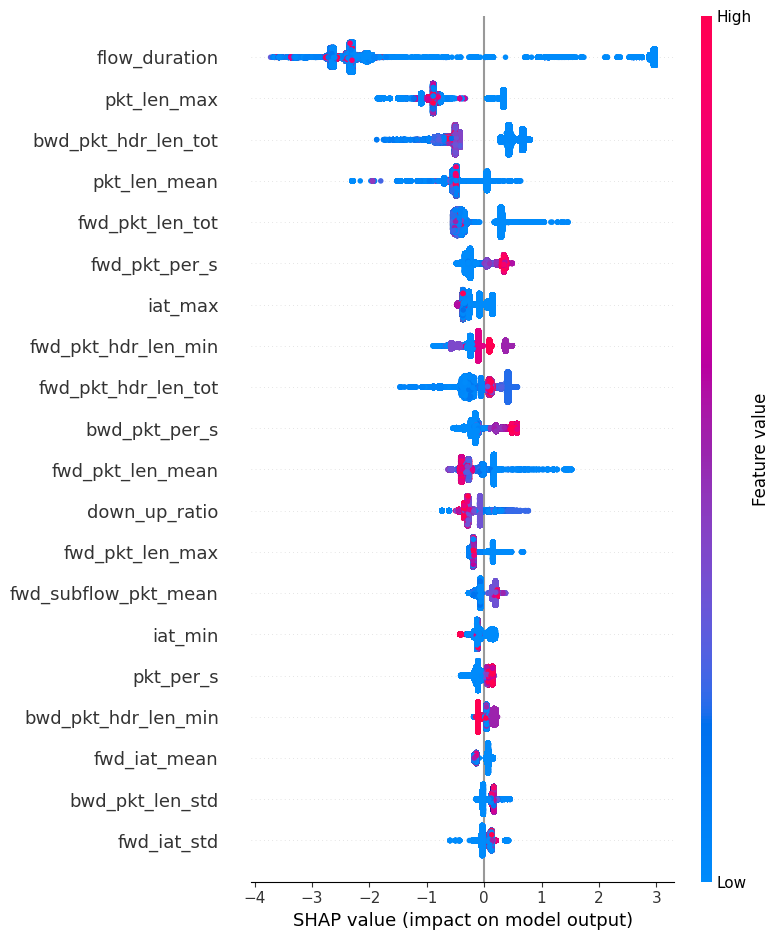
\includegraphics[width=0.8\textwidth]{figures/summary_portscan_criptografado.png}
%     \caption*{Fonte: O autor}
%     \label{fig:summary_portscan_criptografado}
% \end{figure}

% Com base no \emph{dataset} completo, podemos observar que altas taxas de uso da \textit{flag rst} impactam positivamente na classificação de um fluxo como \emph{portscan}, enquanto que a falta deles indica que o fluxo pode não ser desse tipo. Por usar portas de destino raramente utilizadas, os fluxos de \emph{portscan} são facilmente detectados. No entanto, um atacante poderia limitar a faixa de portas escaneadas para evitar ser detectado.

% Esse tipo de ataque também é caracterizado por ter um tempo de duração mais curto. Portanto, fluxos com \textit{flow\_duration} mais altos impactam negativamente na classificação de um fluxo como \emph{portscan}.

% Sem os dados da camada de transporte, a \emph{feature} mais importante para a detecção de \emph{portscan} é a duração do fluxo. Fluxos com \textit{flow\_duration} mais altos impactam negativamente na classificação de um fluxo como \emph{portscan}. Dessa forma, podemos ver que o modelo classifica diversos fluxos como \emph{portscan} apenas por terem durações mais baixas.

\section{Conclusão e trabalhos futuros}
\label{cap:conclusao}

Neste trabalho, foi proposta e implementada uma forma de avaliar a eficácia de modelos de aprendizado de máquina para a detecção de ataques em redes de computadores em situações onde os dados relativos a camada de transporte, como as portas de origem e destino e as \emph{flags} TCP, não estariam disponíveis. Dentre os modelos avaliados, foi possível perceber que a perda de informações da camada de transporte afetou o desempenho dos algoritmos em todas as métricas avaliadas, ainda que em pequena escala. Os resultados foram comparados com os obtidos por \cite{rosay2021cic}, que propuseram uma correção para o \emph{dataset} CIC-IDS2017.

Através da comparação das métricas de \emph{accuracy}, \emph{precision}, \emph{recall}, \emph{f1 score} e MCC, foi possível perceber que os algoritmos, quando usando o conjunto de dados original, obtiveram resultados melhores que todos os modelos avaliados por \cite{rosay2021cic}, porém, quando usando o conjunto de dados criptografado, os resultados foram piores que os obtidos pelo melhor modelo gerado pelos autores. Através da explicabilidade dos modelos, foi possível identificar quais \emph{features} impactam mais na classificação de um fluxo de rede como cada uma das diferentes classes de ataque, o que pode ser útil para a criação de novas técnicas de detecção de ataques e, também, para a criação de técnicas de ataque que evitem a detecção por sistemas de detecção de intrusão baseados em \emph{machine learning}.

Para trabalhos futuros, é possível avaliar a eficácia de outros algoritmos de aprendizado de máquina, assim como diferentes \emph{datasets} para a detecção de ataques em redes de computadores. Além disso, seria interessante avaliar como a criptografia dos dados da camada de transporte afetaria outros protocolos, como o SCTP ou o QUIC.

% \bibliographystyle{abntex2-alf}
% \begin{CJK*}{UTF8}{gbsn}
% \bibliography{biblio}
% \end{CJK*}
\bibliographystyle{sbc}
\bibliography{sbc-template}

\appendix

\end{document}
